\documentclass{article}
\usepackage[margin=0.9in]{geometry}
\usepackage{graphicx}
\usepackage{booktabs}
\usepackage{amsmath}
\usepackage{hyperref}
\usepackage{xcolor}
\usepackage{listings}
\usepackage{caption}
\usepackage{parskip}
\usepackage{enumitem}
\usepackage{longtable}
\usepackage{tabularx}
\setlist{nosep, leftmargin=1.5em}
\hypersetup{colorlinks=true, linkcolor=blue, urlcolor=blue, citecolor=blue}
\lstset{basicstyle=\ttfamily\footnotesize, breaklines=true, columns=fullflexible, frame=single, framerule=0.2pt}
\captionsetup{font=small, labelfont=bf}
\renewcommand{\topfraction}{0.9}
\renewcommand{\bottomfraction}{0.8}
\renewcommand{\textfraction}{0.07}
\renewcommand{\floatpagefraction}{0.85}
\setcounter{topnumber}{3}
\setcounter{totalnumber}{5}
\newcommand{\runcvmedian}{0.4}
\newcommand{\runcvmean}{1.1}
\newcommand{\runcvmax}{10.5}
\newcommand{\runcvmaxpoint}{exp5 write avx512 L2 GB/s}
\newcommand{\runcvn}{48}


\title{Project 2: Cache \& Memory Performance Profiling\\[3pt]\large ECSE 4320/6320 Advanced Computer Systems}
\author{Demetrios Sotirelis}
\date{\today}

\emergencystretch=3em
\begin{document}
\maketitle

\begin{abstract}
This report characterizes the memory hierarchy of an AMD Ryzen~9 9950X, a Zen~5 processor with dual-channel double data rate 5 (DDR5) memory at 6000 megatransfers per second. Dependent pointer chases measure zero-queue latency, streaming kernels using Advanced Vector Extensions 512 (AVX-512) measure bandwidth, and a loaded-latency method modelled on Intel's Memory Latency Checker (MLC) measures latency under load. Latency rises from 4 cycles in L1 to about 500 cycles, or 89\,ns, in dynamic random-access memory (DRAM). One core streams 58\,GB/s from DRAM; 14 cores reach about 70\,GB/s, 73\% of the theoretical rate, where latency has doubled and Little's Law gives about 190 cache lines in flight. Dependent, independent and sequential access cause the same DRAM misses but differ 40--80 times in cost, and a model built from four hardware-counter events reproduces the measured latency within 22\%. With 2\,MiB huge pages the translation lookaside buffer (TLB) penalty almost disappears. Nine benchmark pitfalls are measured. A summary of results, a map from the grading rubric to this report and a requirements checklist are in the appendices.
\end{abstract}

\section{Reproducibility}\label{sec:repro}
The repository holds the sources (\texttt{src/}), the scripts (\texttt{scripts/}), the raw measurements (\texttt{data/raw}, \texttt{data/repeats}), the derived tables (\texttt{data/processed}) and the figures with the recorded environment, clock log and build flags (\texttt{results/}). The commands below rebuild everything.
\begin{lstlisting}
powershell -File scripts\build.ps1                 # builds bin\*.exe (flags in results\build_flags.txt)
powershell -File scripts\run_all.ps1               # all experiments -> data\raw (+ results\environment.txt, frequency_log.csv)
powershell -File scripts\run_all.ps1 -RawDir data\repeats\run2 -Subset     # repeats (also run3)
python scripts\process_and_plot.py                 # raw -> data\processed, results\fig*.png, report\generated\*.tex
python scripts\repeat_check.py                     # run-to-run variation
powershell -File scripts\run_counters.ps1         # elevated shell: hardware counters -> data\raw\counters\exp9_counters.csv
python scripts\process_counters.py                # counters -> results\figE_counters.png, report\generated\table_counters_*.tex
\end{lstlisting}
To measure run-to-run variation, the headline experiments ran in three independent processes, and \nolinkurl{scripts/repeat_check.py} compares \runcvn\ summary points. The median coefficient of variation is \runcvmedian\%. The largest variation, 10\%, is the single-core L2 write bandwidth, which depends on where the L2 holds dirty lines; every conclusion rests on points that vary by less than 3\%.

\section{Methodology}\label{sec:method}
\subsection{Platform}\label{sec:platform}
{\small
\begin{longtable}{p{2.6cm}p{13.4cm}}
\toprule
Processor & AMD Ryzen 9 9950X, 16 cores with simultaneous multithreading (SMT) enabled, on two 8-core core complex dies (CCDs), with logical processors 0--15 on the first and 16--31 on the second and SMT siblings adjacent \\
Memory & 2 $\times$ 16\,GB of DDR5 memory at 6000\,MT/s, dual channel, 96\,GB/s theoretical; a single non-uniform memory access (NUMA) node \\
Software & Windows 11 build 26200; g++ 16.2.0 from MinGW-w64 with \texttt{-O3 -march=native -static}; Python 3.12 \\
Frequency & High performance power plan, recorded but not changed. A dependent-add chain measures 5.64\,GHz on logical processor 4 and 5.46\,GHz on the second CCD; cycle values use the clock of the run's pinned core. The clock of the loaded runs' cores was not measured. \\
Pinning & Single-core experiments on logical processor 4 with its SMT sibling idle, at high priority. Loaded-latency experiments put one generator thread on each of physical cores 0--13, the latency probe on core 14 and the controller on core 15, with SMT siblings idle; about 1\% background load. \\
Huge pages & 2\,MiB pages only for the huge-page arm (exp7) and the huge-page counter runs; every other experiment uses 4\,KiB pages. The user account holds the ``Lock pages in memory'' right, and the program enables it in its own process only \cite{mslarge}. \\
Data & Memory written before timing; random addresses precomputed; each chase node is one 64\,B line holding the offset of the next. Plots show the median and the interquartile range. \\
\bottomrule
\end{longtable}
}

\subsection{Measurement methods}\label{sec:methods}
A dependent pointer chase measures zero-queue latency. It follows a single random cycle through 64\,B nodes, so only one load is in flight and no prefetcher can follow it. Each value is the median of 5--7 repetitions of $10^6$ timed hops after an untimed warm-up. Cycles are ns times the clock measured on the pinned core during the run, never the nominal clock. With 4\,KiB pages the DRAM value includes a page walk.

AVX-512 streaming kernels with integer accumulators measure bandwidth by reading or writing private buffers; batches are doubled to at least 8\,ms, with 7 repetitions.

Loaded latency comes from an equivalent of Intel's MLC \cite{intelmlc}, which was not run. Up to 14 generator threads stream a chosen read/write mix over private 512\,MiB regions, with the intensity set by the thread count and an injected delay after every 40\,KiB chunk, while the probe thread runs the dependent chase on its own buffer. Each point has a 0.3\,s warm-up and a 0.6\,s window, with 4 repetitions.

\subsection{Hardware counters}\label{sec:countermethod}
Windows has no \texttt{perf}, but Event Tracing for Windows (ETW) logs the performance counters at every context switch. Windows Performance Recorder (WPR) records the trace and \texttt{tools/etl\_pmc.cpp} decodes it, so nothing is installed and no setting changes; ETW kernel tracing does need an elevated session. Each target is pinned to logical processor 4 and run twice with different iteration counts; differencing the two removes allocation and setup, and runs were repeated only where results varied. The counters are cycles, retired instructions, L1 data cache (L1D) fills by source and misses in the first-level data TLB (DTLB), using the Zen~5 event codes of the Linux perf tables \cite{perfzen5}. Their ``L3'' source also counts fills from another L2 in the same core complex, which cannot occur for one pinned core. Counts include prefetch and page-walk traffic, and there are no memory-controller counters, so DRAM row hits and bus turnarounds are not measured.

The counters were validated on cases with a known answer. The L1-resident chase takes exactly 4 cycles per hop, confirming the measured clock; the 64--512\,KiB chase shows exactly one L2 fill per hop; and DTLB misses grow with the page count. Two traps found on the way are pitfall~7 (Sec.~\ref{sec:pitfalls}).

\subsection{Correctness validation}\label{sec:valid}
Every chase layout is one cycle through all nodes, and \texttt{Chase::verify()} re-walks it for every measured configuration. The layout of the TLB experiment has no duplicate lines, so the cache footprint really is constant, and the mix kernel performs exactly $R$ reads and $10-R$ writes per 10 lines. Bandwidth kernels are checked before timing against scalar sums for reads and byte-wise checks for stores, including non-temporal ones.

The results also agree with the hardware. The 4-cycle L1 latency matches the value reported for Zen~5 \cite{amdhc}; no published L2 latency was found, so the 14 cycles rest on the counters. The naive floating-point sum runs at exactly one 4-byte add per 2 cycles, and one core and eight cores of one CCD reach the same plateau in DRAM. As cross-checks, the loaded probe's idle latency matches the single-thread chase, and Little's Law is checked two ways (Sec.~\ref{sec:knee}).

\section{Hypotheses}\label{sec:hyp}
{\small
\begin{longtable}{@{}lp{7.7cm}p{7.7cm}@{}}
\toprule
& \textbf{Prediction} & \textbf{Outcome} \\
\midrule
\endhead
1 & The benchmark will observe a latency staircase effect. Increasing from around 5 cycles to 80ns as we push up from L1 cache to DRAM. Steps will be observed around the cache capacities of 48\,KiB, 1\,MiB and less than 32\,MiB for L3, as L3 is shared. AMD gives 4 cycles for L1 \cite{amdhc}; $\frac{0.5}{6000 \text{MHz}} \approx 80\text{ns}$ for DRAM. & Held, with 4, 14 and 49 cycles and 89\,ns from L1, L2 and L3 to DRAM; the L3 step comes at about 24\,MiB (Sec.~\ref{sec:zq}). \\
2 & One core is limited by the line fills it keeps in flight, so DRAM bandwidth rises with threads until the memory controller saturates. & Hypothesis not observed. One core already saturates its core complex's DRAM bandwidth, which means no thread scaling with locality. The prefetcher makes even 4\,KiB strides (Sec.~\ref{sec:sweeps}) cheap. \\
3 & Write-allocate and write-back make writes cost more, so pure reads are fastest and pure writes slowest. & Held (Sec.~\ref{sec:mix}). \\
4 &  Flat until a knee, then rising steeply with no more throughput; Little's Law gives a constant maximum concurrency at saturation. Requests queue at the memory controller, so until it saturates more requests add throughput, and after that they only wait. & Held (Sec.~\ref{sec:knee}). \\
5 & Dependent cache and TLB misses serialize while independent misses overlap through memory-level parallelism (MLP). Spreading a fixed footprint over more pages adds latency once the TLB's reach is exceeded, and 2\,MiB pages remove most of it. & Held; the huge-page saving on a 1\,GiB chase exceeded the translation share the counter model predicts (Sec.~\ref{sec:counters}, \ref{sec:tlb}). \\
6 & In the hardware counters, the fills from each level determine the latency of a dependent load, DTLB misses add a cost that grows with the page count, and miss counts do not predict the runtime of independent loads. & Held (Sec.~\ref{sec:counters}). \\
\bottomrule
\end{longtable}
}

\section{Results}\label{sec:results}
\subsection{Zero-queue latency and working-set sweep}\label{sec:zq}
\begin{table}[!htb]\centering\small\resizebox{\linewidth}{!}{\begin{tabular}{llrrrrr}
\toprule
level & footprint band & random ns & page-blocked ns & random cycles & page-blocked cycles & random ns (CPU 20) \\
\midrule
L1 & 4 KiB--32 KiB & 0.72 & 0.72 & 4 & 4 & 0.73 \\
L2 & 128 KiB--768 KiB & 2.48 & 1.60 & 14 & 9 & 2.56 \\
L3 & 2 MiB--8 MiB & 8.74 & 3.59 & 49 & 20 & 9.01 \\
DRAM & 512 MiB--1 GiB & 89.11 & 27.83 & 503 & 157 & 92.84 \\
\bottomrule
\end{tabular}
}
\caption{Per-level latency, median over each footprint band, in ns and in cycles at 5.64\,GHz. ``Random'' is the dependent chase over random lines, the zero-queue latency; ``page-blocked'' visits all 64 lines of a page before moving on (pitfall~5).}\label{tab:latency}\end{table}
\begin{figure}[!htb]\centering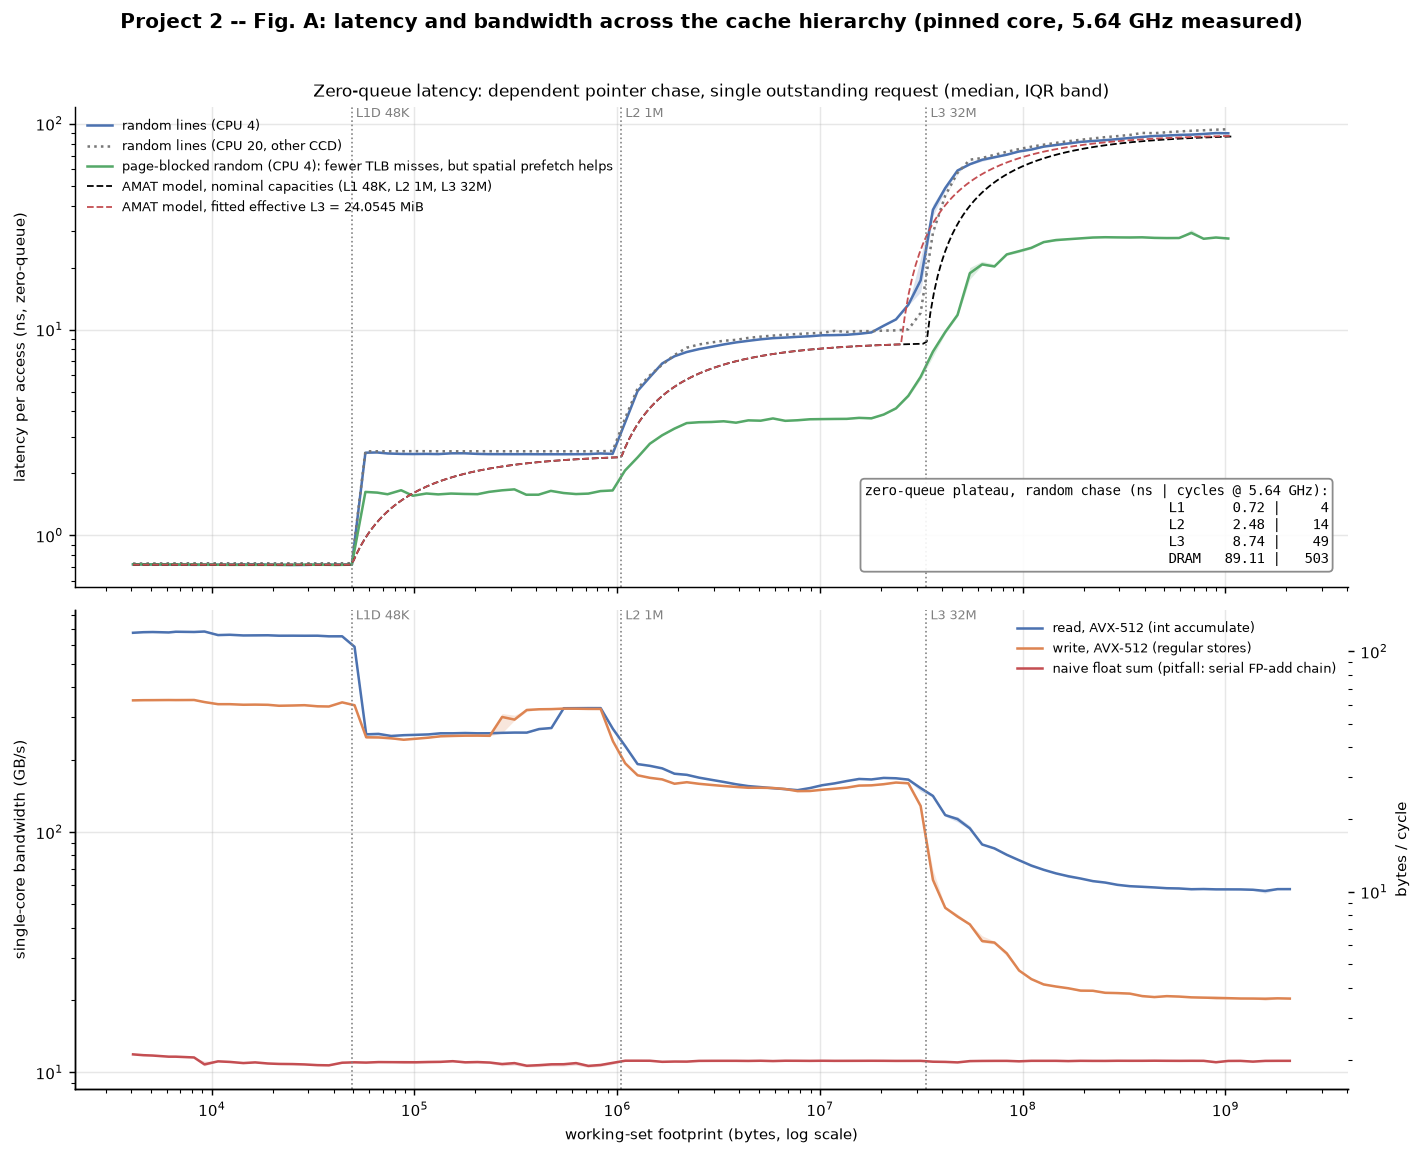
\includegraphics[width=0.9\linewidth]{../results/figA_latency_and_workingset.png}
\caption{Dependent random chase on two cores, one on each core complex, with the page-blocked variant and the average-memory-access-time models (top); single-core read and write bandwidth and the naive floating-point sum (bottom). Dotted lines mark the nominal L1D, L2 and L3 capacities.}\label{fig:A}\end{figure}
Latency rises in clear steps at the capacities of L1D, L2 and L3 (Tab.~\ref{tab:latency}, Fig.~\ref{fig:A}). Cores on the second CCD are a few percent slower in ns because they run a 3\% lower clock; in cycles they match. Chips and Cheese report just over 70\,ns of memory latency for a 9950X at the same memory speed \cite{chips9950x}; the chase here gives 89\,ns on 4\,KiB pages and 79\,ns on 2\,MiB pages, with different memory timings and method. Within the L3 band latency drifts upward with the footprint; huge pages show that about 40\% of this drift is address translation and the rest is the L3 itself (Sec.~\ref{sec:tlb}).

An average memory access time (AMAT) model \cite{hennessy}, which weights each level's latency by the fraction of the footprint that fits in it, matches the plateaus, but the measured steps are sharper. A chase repeats the same cycle, the worst case for a least-recently-used cache, so the miss rate jumps to nearly 100\% once the cycle no longer fits. The L3 capacity that best fits the curve is about 24\,MiB, three quarters of nominal; the counters confirm it (Sec.~\ref{sec:counters}), but the cause is open (Sec.~\ref{sec:anomalies}).

\subsection{Bandwidth, access pattern and granularity}\label{sec:sweeps}
\begin{table}[!htb]\centering\small\begin{tabular}{lrrrrrr}
\toprule
 & \multicolumn{2}{c}{read (AVX-512)} & \multicolumn{2}{c}{write (AVX-512)} & \multicolumn{2}{c}{naive FP sum (pitfall)} \\
level & GB/s & B/cycle & GB/s & B/cycle & GB/s & B/cycle \\
\midrule
L1 & 682.4 & 121.0 & 354.2 & 62.8 & 11.9 & 2.11 \\
L2 & 327.5 & 58.1 & 326.0 & 57.8 & 11.1 & 1.98 \\
L3 & 173.0 & 30.7 & 161.2 & 28.6 & 11.2 & 1.98 \\
DRAM & 57.8 & 10.2 & 20.4 & 3.6 & 11.2 & 1.98 \\
\bottomrule
\end{tabular}

\caption{Single-core bandwidth per level, the maximum over each footprint band, with DRAM at 512\,MiB or more. The last pair is the naive floating-point sum of pitfall~2.}\label{tab:bw}\end{table}
\begin{figure}[!htb]\centering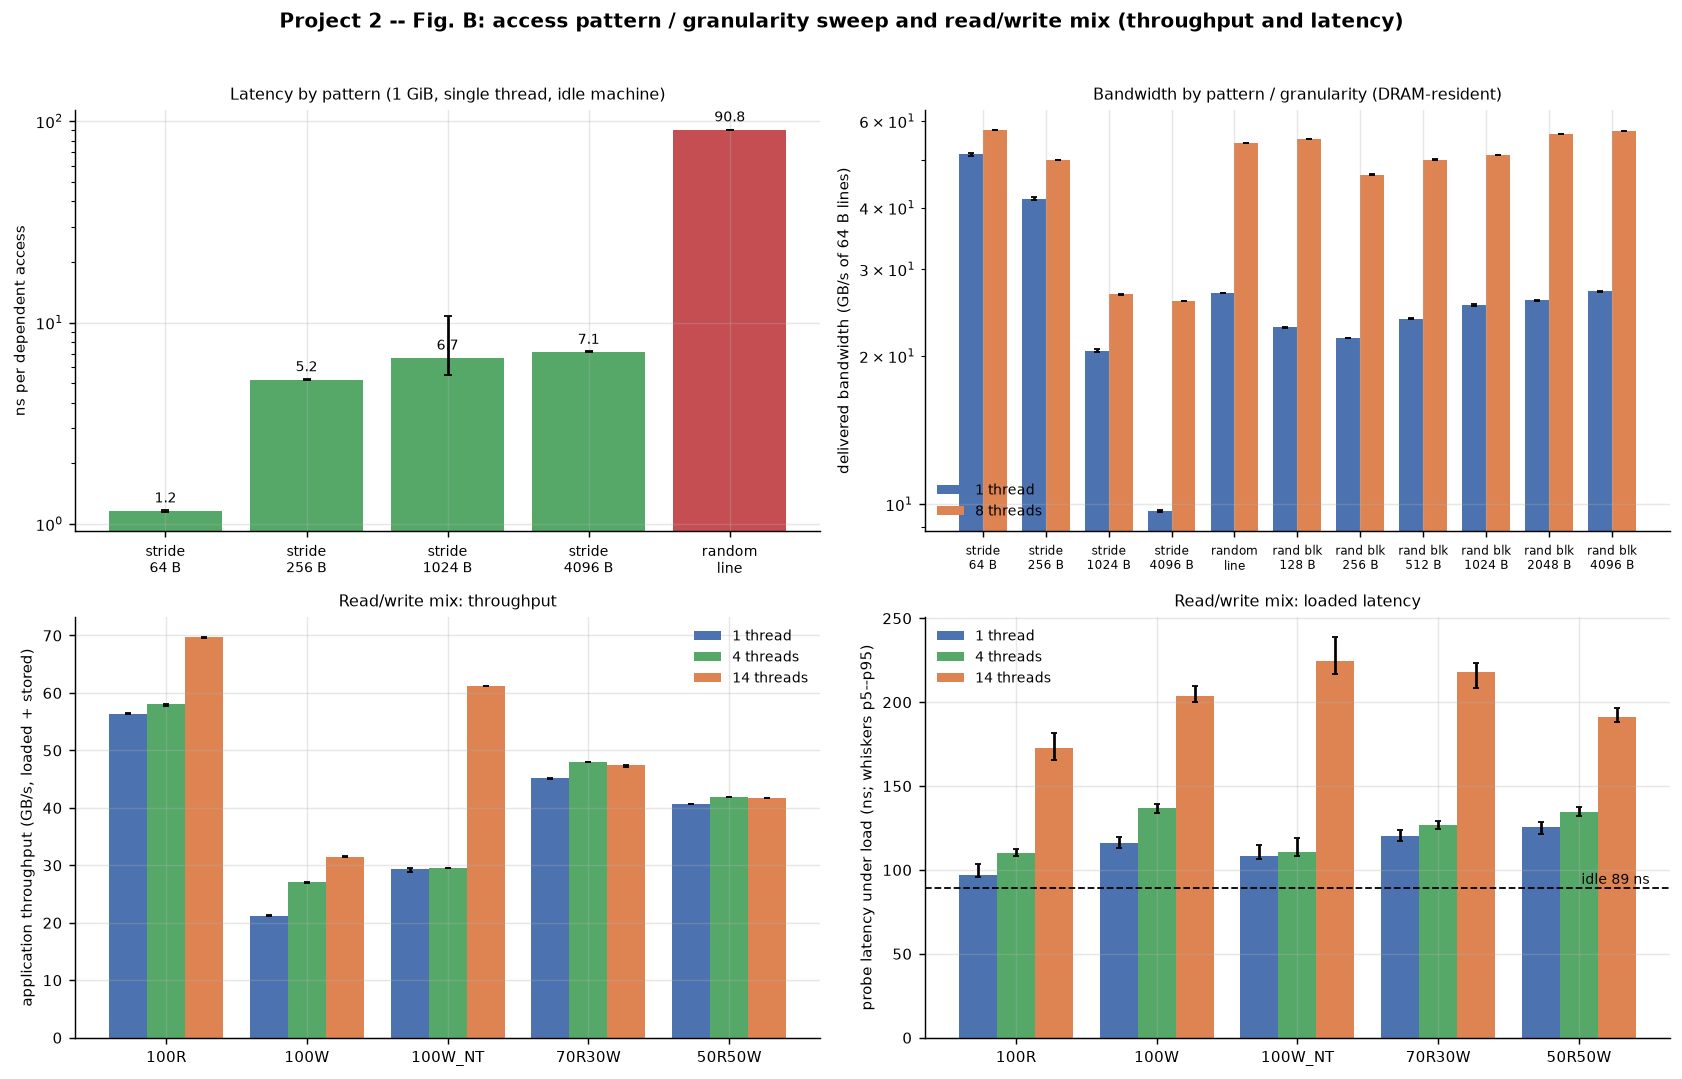
\includegraphics[width=\linewidth]{../results/figB_pattern_granularity_and_rwmix.png}
\caption{Latency of a 1\,GiB dependent chase and bandwidth over a private 512\,MiB buffer per thread, by pattern and granularity, for 1 and 8 threads (top); application throughput and probe latency for each read/write mix with 1, 4 and 14 threads (bottom).}\label{fig:B}\end{figure}
One core reads about 120 bytes per cycle from L1, roughly halving at each level to about 10 from DRAM (Tab.~\ref{tab:bw}). In DRAM, regular stores reach only a third of the read rate, because each store first reads its line, called write-allocate, and later writes it back.

The hardware prefetcher follows a dependent chase with a fixed stride, so strides up to 4\,KiB cost only a few ns per load, against 91\,ns for random lines (Fig.~\ref{fig:B}). Bandwidth follows the number of lines a core keeps in flight. One thread streams sequential data at nearly the core complex's DRAM limit, and larger strides deliver less because each access needs a new line or page. Random lines reach about half the sequential rate with one thread and come within 6\% of it with 8 threads. With enough independent requests outstanding, random access is limited by bandwidth, not latency.

Larger random blocks amortize the first-line miss and engage the streaming prefetcher. Eight threads on one core complex plateau at the single-core sequential rate, so the limit is the core complex's link to the memory controller, not the cores.

\subsection{Read/write mix}\label{sec:mix}
\begin{table}[!htb]\centering\small\begin{tabular}{lrrrrr}
\toprule
mix & threads & GB/s & probe p50 ns & p5--p95 ns & DRAM bus est. GB/s \\
\midrule
100R & 1 & 56.3 & 97 & 96--104 & 56.3 \\
100R & 14 & 69.7 & 173 & 166--182 & 69.7 \\
100W & 1 & 21.3 & 116 & 113--119 & 42.5 \\
100W & 14 & 31.5 & 203 & 200--209 & 63.0 \\
100W\_NT & 1 & 29.4 & 108 & 107--115 & 29.4 \\
100W\_NT & 14 & 61.2 & 224 & 217--239 & 61.2 \\
70R30W & 1 & 45.2 & 120 & 117--124 & 58.7 \\
70R30W & 14 & 47.4 & 218 & 208--224 & 61.6 \\
50R50W & 1 & 40.6 & 126 & 122--129 & 60.9 \\
50R50W & 14 & 41.8 & 191 & 188--197 & 62.6 \\
\bottomrule
\end{tabular}

\caption{Read/write mixes at maximum intensity. The DRAM-bus estimate adds one write-allocate read per line stored with regular stores; non-temporal stores avoid it.}\label{tab:mix}\end{table}
With 14 threads on both core complexes, pure reads are fastest, but every mix moves about the same estimated DRAM-bus traffic once write-allocate reads are added (Tab.~\ref{tab:mix}, Fig.~\ref{fig:B} bottom); the bus traffic is not measured directly. Pure reads are about 10\% more efficient because the bus never switches direction. Non-temporal stores bypass the caches and skip the write-allocate read, doubling write throughput. Every mix with writes raises the probe latency above that of pure reads.

\subsection{Throughput--latency knee}\label{sec:knee}
\begin{figure}[!htb]\centering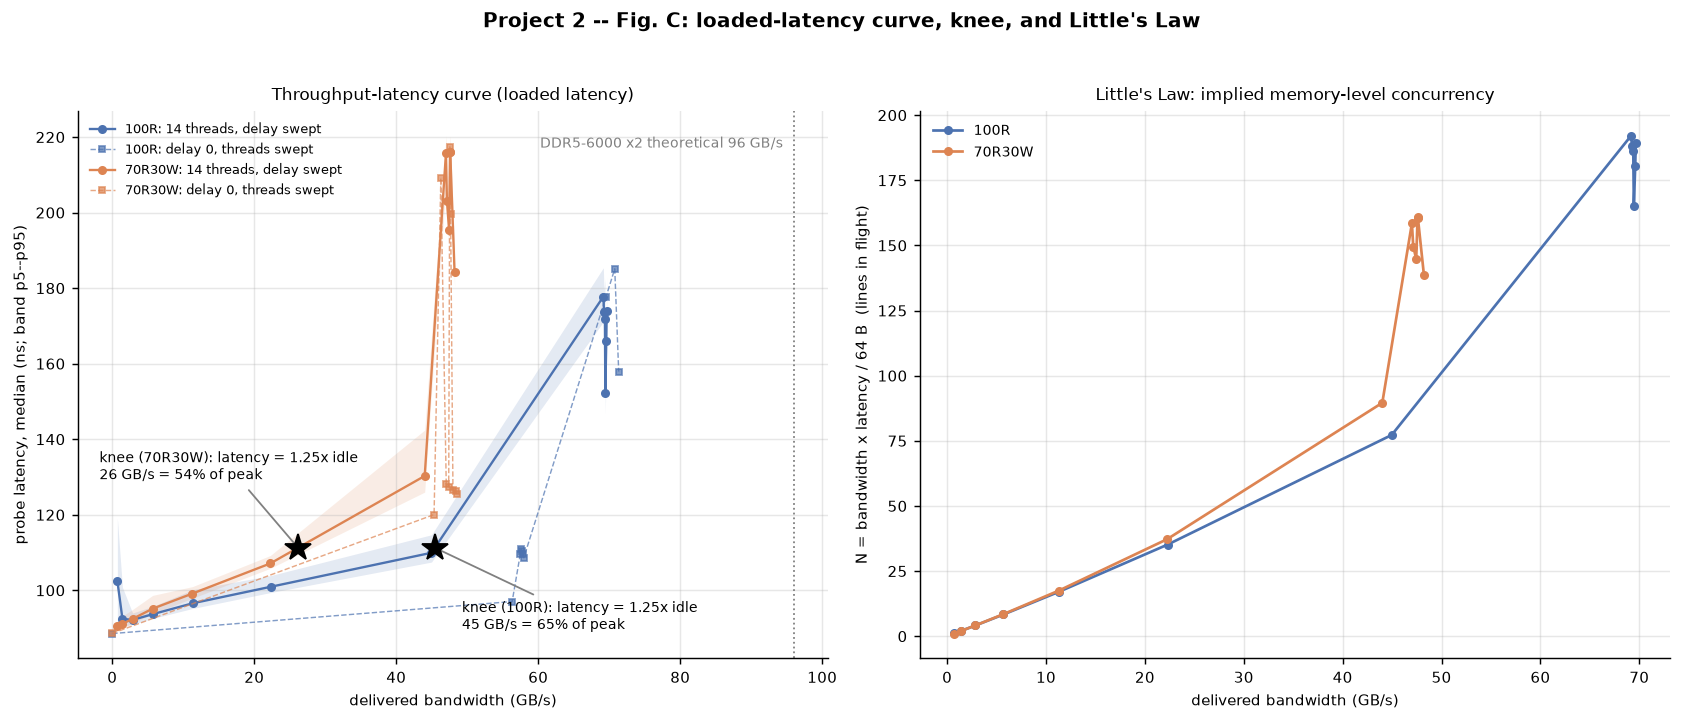
\includegraphics[width=\linewidth]{../results/figC_loaded_latency_curve.png}
\caption{Probe latency against delivered bandwidth (left) as the generators' injected delay falls from 800\,$\mu$s to zero with 14 threads, and, dashed, with zero delay and 0--14 threads, for pure reads and the 70/30 mix, and the implied concurrency $N=\text{BW}\times\text{latency}/64\,\text{B}$ (right).}\label{fig:C}\end{figure}
\begin{table}[!htb]\centering\small\resizebox{\linewidth}{!}{\begin{tabular}{lrrrrrrrr}
\toprule
mix & idle ns & BW at 1.25$\times$ idle (knee) & BW at 1.5$\times$ & peak GB/s & ns at peak & latency $\times$ & $N$ at knee & $N$ at peak \\
\midrule
100R & 89 & 45.4 (65\%) & 53.4 (77\%) & 69.6 & 173 & 1.94 & 79 & 188 \\
70R30W & 89 & 26.2 (54\%) & 44.1 (92\%) & 48.2 & 209 & 2.35 & 45 & 158 \\
\bottomrule
\end{tabular}
}
\caption{Knee, the interpolated bandwidth at which latency reaches 1.25$\times$ and 1.5$\times$ idle, and saturation. $N$ is the number of lines in flight from Little's Law.}\label{tab:knee}\end{table}
The curve has the classic queueing shape (Fig.~\ref{fig:C}). Latency stays within 10\% of idle up to about 11\,GB/s, then rises, and near saturation throughput stops growing while latency keeps rising. The knee is defined as the bandwidth at which latency reaches 1.25$\times$ idle, which is about two thirds of peak for pure reads and half of peak for the 70/30 mix (Tab.~\ref{tab:knee}). From the knee to saturation, throughput and latency both grow by about half; past saturation, latency grows another 16\% with no bandwidth gain. The peak is 73\% of the theoretical 96\,GB/s.

Little's Law \cite{little1961} gives the concurrency behind the delivered bandwidth, $N=\mathrm{BW}\times\mathrm{latency}/64\,\mathrm{B}$, using the probe's latency on the assumption that generator requests see the same queueing delay. Below the knee, $N$ grows at nearly constant latency because the cores issue more requests; at saturation the memory controller queues them, and extra concurrency only adds waiting. The cores are not the limit, since one core alone sustains about 40 lines in flight (Sec.~\ref{sec:counters}), while 14 cores at the DRAM limit need only about 13 each. The 70/30 mix saturates earlier and at higher latency, because writes take bus time without adding delivered bandwidth.

\subsection{Cache misses and hardware counters}\label{sec:counters}
\begin{figure}[!htb]\centering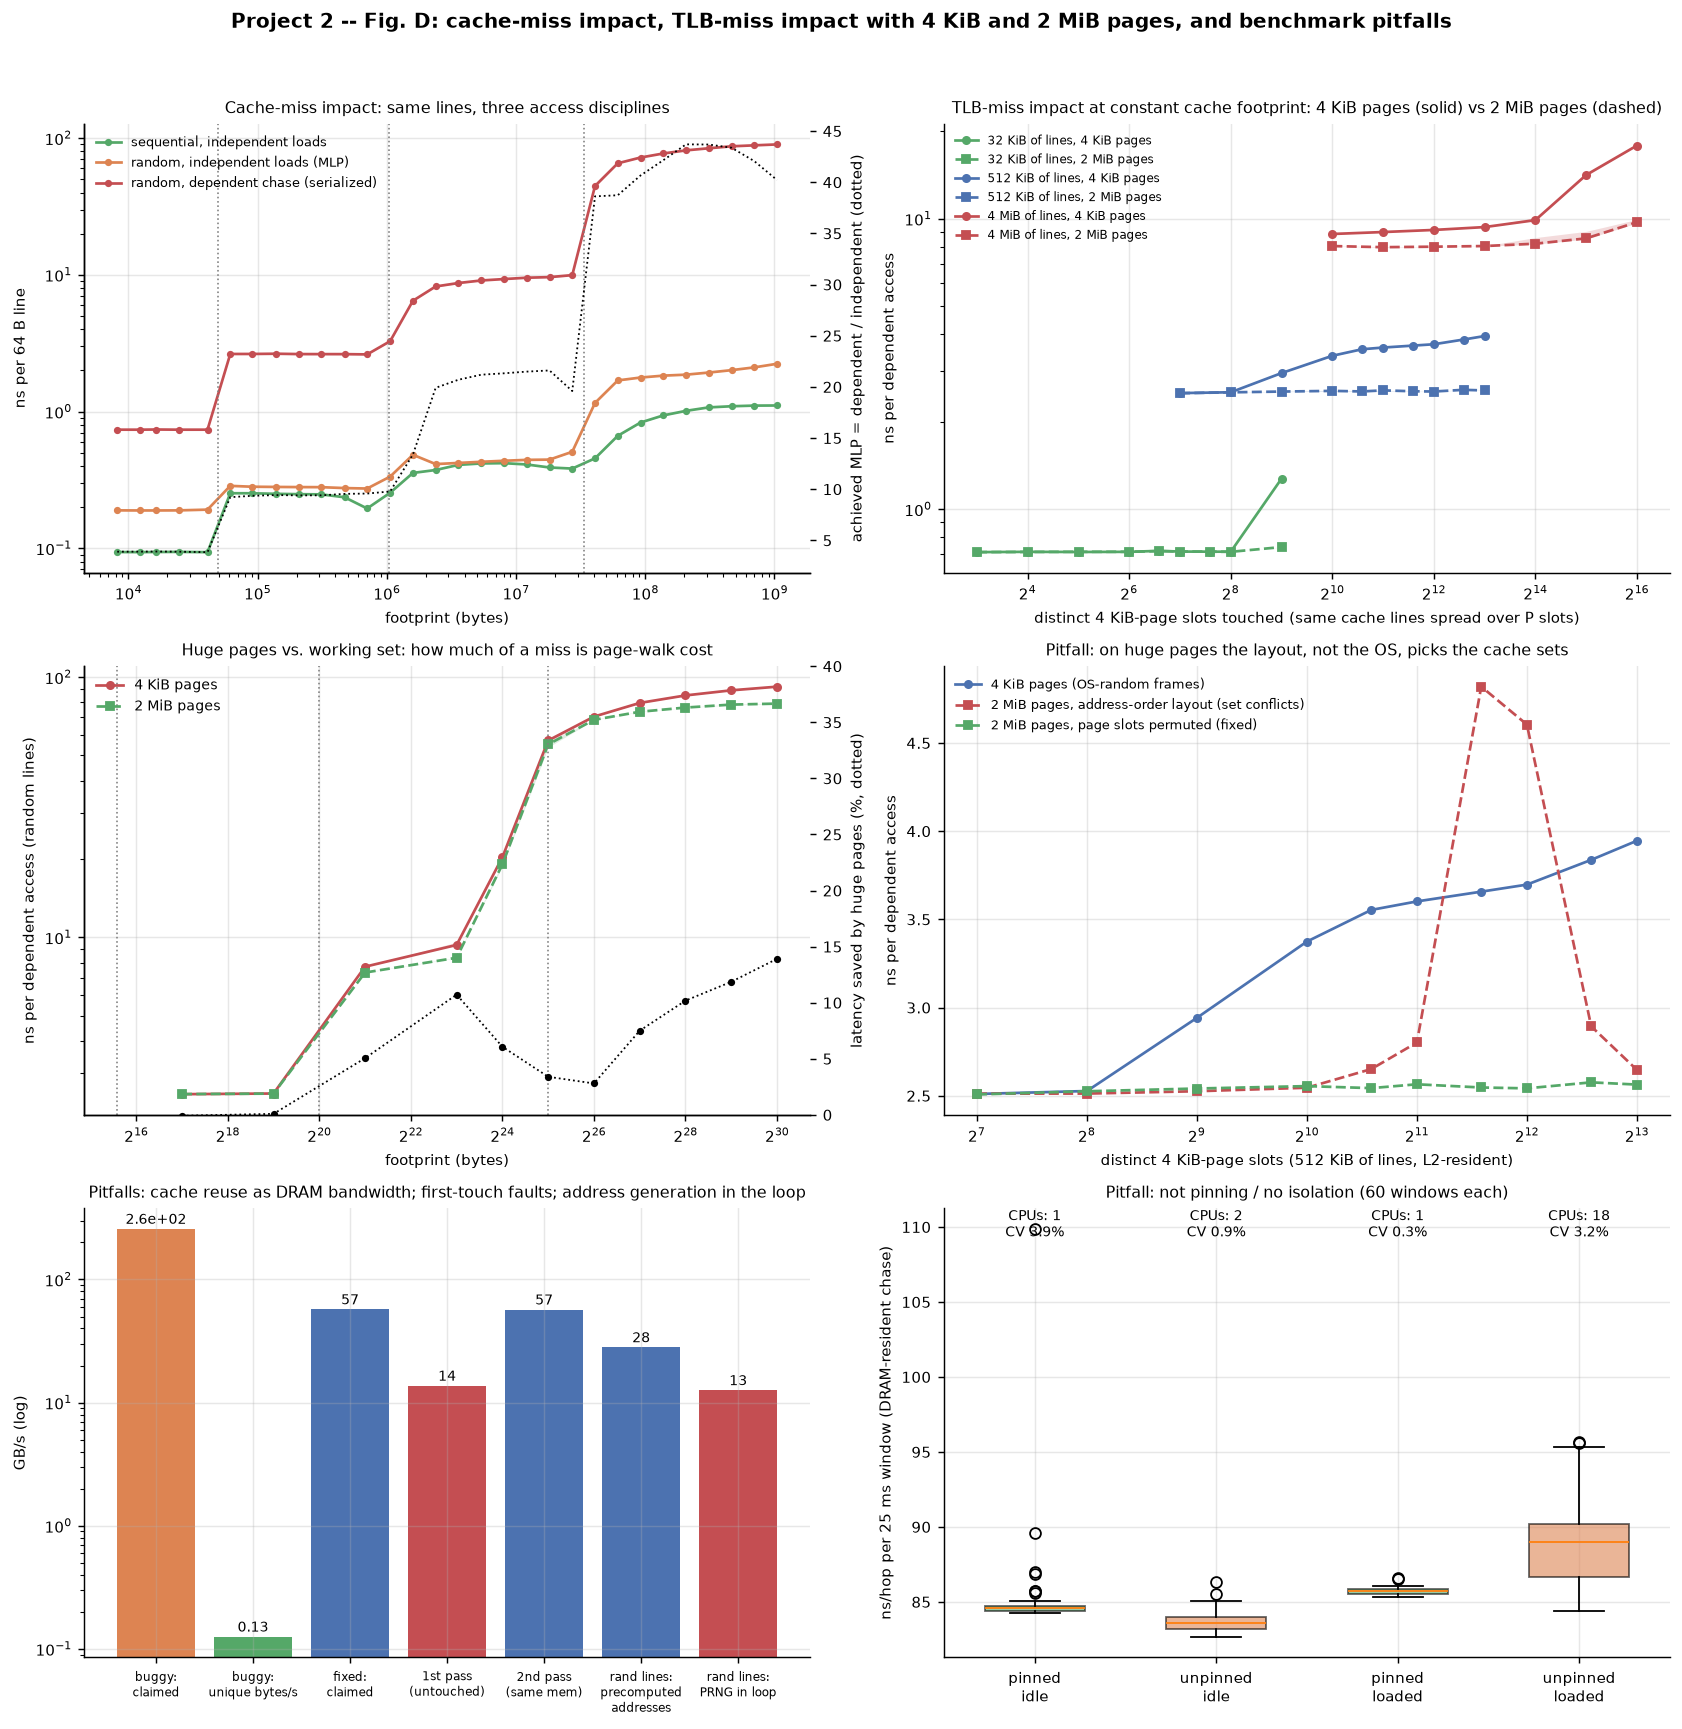
\includegraphics[width=0.88\linewidth]{../results/figD_cachemiss_tlbmiss_and_pitfall.png}
\caption{The same lines touched three ways, with the achieved MLP dotted, and the constant-footprint TLB experiment on 4\,KiB pages, solid, and 2\,MiB pages, dashed (row 1); dependent chase over random lines against footprint on both page sizes, with the latency saved by huge pages dotted, and the huge-page layout pitfall (row 2); benchmark pitfalls and the effect of not pinning (row 3).}\label{fig:D}\end{figure}
\begin{table}[!htb]\centering\small\resizebox{\linewidth}{!}{\begin{tabular}{rrrrrrrr}
\toprule
footprint & ns/hop & cycles & instr. & fills from L2 & from L3 & from DRAM & DTLB miss \\
 & & per hop & per hop & per hop & per hop & per hop & per hop \\
\midrule
16 KiB & 0.71 & 4.0 & 2.50 & 0.000 & 0.000 & 0.000 & 0.000 \\
32 KiB & 0.71 & 4.0 & 2.51 & 0.000 & 0.000 & 0.000 & 0.000 \\
64 KiB & 2.50 & 14.0 & 2.50 & 1.000 & 0.000 & 0.000 & 0.000 \\
256 KiB & 2.49 & 14.0 & 2.50 & 1.000 & 0.000 & 0.000 & 0.000 \\
512 KiB & 2.49 & 14.1 & 2.51 & 1.000 & 0.000 & 0.000 & 0.000 \\
1024 KiB & 2.97 & 16.4 & 2.50 & 0.934 & 0.066 & 0.000 & 0.001 \\
4096 KiB & 8.83 & 49.3 & 2.51 & 0.095 & 0.906 & 0.000 & 0.640 \\
8192 KiB & 9.94 & 37.9 & 2.52 & 0.041 & 0.991 & -0.034 & 0.820 \\
16384 KiB & 18.90 & 107.7 & 2.54 & 0.021 & 0.853 & 0.127 & 0.910 \\
32768 KiB & 52.83 & 295.0 & 2.60 & 0.025 & 0.394 & 0.601 & 0.955 \\
65536 KiB & 71.58 & 402.9 & 2.64 & 0.047 & 0.132 & 0.875 & 0.979 \\
262144 KiB & 84.83 & 477.7 & 2.71 & 0.459 & 0.329 & 0.970 & 0.996 \\
1048576 KiB & 90.82 & 511.5 & 2.71 & 0.195 & 0.772 & 0.995 & 1.001 \\
\bottomrule
\end{tabular}
}
\caption{Dependent pointer chase over compact 4\,KiB pages, with L1D fills per hop by the level that served them. One run per row, three for 4--64\,MiB, whose result depends on the physical pages the operating system hands out.}\label{tab:cchase}\end{table}
\begin{table}[!htb]\centering\small\begin{tabular}{lrr}
\toprule
term of the model $t = t_0 + \sum_i n_i c_i$ & fitted $c_i$ (ns) & cycles at 5.64\,GHz \\
\midrule
base: L1 hit (load-to-use) & 0.71 & 4 \\
extra per L1D fill from L2 & 1.80 & 10 \\
extra per L1D fill from L3 & 8.66 & 49 \\
extra per L1D fill from DRAM & 78.32 & 442 \\
extra per DTLB miss & 1.37 & 8 \\
\bottomrule
\multicolumn{3}{l}{\footnotesize weighted least squares over 25 configurations: median error 1\%, maximum 22\%, $R^2$ (log scale) $=0.998$}\\
\end{tabular}

\caption{Cost of each counted event, $t = t_0 + \sum_i n_i c_i$, fitted by weighted least squares to the 25 chase configurations of Tab.~\ref{tab:cchase} and the TLB runs.}\label{tab:cfit}\end{table}
\begin{table}[!htb]\centering\small\begin{tabular}{lrrrrrr}
\toprule
1 GiB of lines, touched\ldots & ns/line & cycles & instr. & DRAM fills/line & DTLB miss/line & implied MLP \\
\midrule
dependent chase & 90.08 & 509.3 & 2.70 & 0.992 & 1.001 & 1 \\
independent random & 2.23 & 12.5 & 3.76 & 1.010 & 1.043 & 40 \\
sequential & 1.12 & 6.3 & 2.50 & 0.983 & 0.005 & 81 \\
\bottomrule
\end{tabular}

\caption{The same 1\,GiB of cache lines, each touched once in three ways. Implied MLP is the dependent time per line divided by the time per line.}\label{tab:cdisc}\end{table}
\begin{table}[!htb]\centering\small\resizebox{\linewidth}{!}{\begin{tabular}{llrrrrrrr}
\toprule
kernel & footprint (3 arrays) & ns/elem & cycles/elem & fills L2 / L3 / DRAM per elem & line-fill traffic (B/elem) & DTLB miss/elem & instr./elem \\
\midrule
mul & 48 KiB & 0.0201 & 0.108 & 0.0019 / 0.0000 / 0.0000 & 0.12 & 0.0000 & 0.379 \\
mul & 768 KiB & 0.0374 & 0.195 & 0.1872 / 0.0000 / 0.0000 & 12.00 & 0.0000 & 0.375 \\
mul & 12288 KiB & 0.0754 & 0.388 & 0.1856 / 0.0028 / 0.0000 & 12.03 & 0.0008 & 0.375 \\
mul & 393216 KiB & 0.2622 & 1.468 & 0.0197 / 0.0000 / 0.1700 & 12.16 & 0.0008 & 0.376 \\
saxpy & 48 KiB & 0.0203 & 0.110 & 0.0000 / 0.0000 / 0.0000 & 0.00 & 0.0000 & 0.391 \\
saxpy & 768 KiB & 0.0259 & 0.130 & 0.1252 / 0.0000 / 0.0000 & 8.01 & 0.0000 & 0.376 \\
saxpy & 12288 KiB & 0.0595 & 0.341 & 0.1178 / -0.0031 / 0.0098 & 7.97 & 0.0006 & 0.375 \\
saxpy & 393216 KiB & 0.1872 & 1.052 & 0.0380 / 0.0000 / 0.0875 & 8.05 & 0.0006 & 0.375 \\
\bottomrule
\end{tabular}
}
\caption{The course document's simple float32 kernels, $z=x\cdot y$ and $y=a\cdot x+y$, auto-vectorized for AVX-512 over three arrays, with counters per element. Line-fill traffic is 64\,B times the fills from L2, L3 and DRAM.}\label{tab:ckern}\end{table}
Touching the same lines once per pass costs least with sequential loads, about twice as much with random independent loads and far more with random dependent loads (Fig.~\ref{fig:D}, top left). The ratio of dependent to independent cost, the achieved MLP, grows from about 4 in L1 to about 40 in DRAM. With independent addresses a core overlaps about 40 misses and exposes only a fortieth of the DRAM latency per line. The three patterns cause the same number of DRAM misses per line, yet their costs differ by 40 and 80 times (Tab.~\ref{tab:cdisc}), so miss counts alone do not determine time. The address-generation pitfall (Sec.~\ref{sec:pitfalls}) matters for the same reason, because it changes cycles and instructions per line, not the miss count.

Up to 32\,KiB every load hits L1, and from 64 to 512\,KiB every load is served by L2 (Tab.~\ref{tab:cchase}). From 4\,MiB most loads come from L3, and DTLB misses rise as the footprint outgrows the TLB's reach. DRAM fills appear at 16\,MiB and dominate from 64\,MiB, so the L3 holds the whole chase only up to 8--16\,MiB and half of it near 28\,MiB, confirming the effective capacity of about 24\,MiB. The counters show that only part of the L3 is usable, not why; untested candidates are its replacement policy under a cyclic pattern and its role as the L2's victim cache.

The counters also explain the latency. A linear model in the four counted events, fitted to minimize relative error, reproduces all 25 configurations within 22\%, with a median error of 1\% (Tab.~\ref{tab:cfit}). This is AMAT with measured rather than inferred event counts, and its terms agree with the zero-queue table, since an L1 hit plus one L2 fill gives the 14-cycle L2 latency. In a 1\,GiB chase each hop also walks the page table, whose entries come from L2 and L3, so by this model about 9\% of the DRAM latency on 4\,KiB pages is address translation.

For single-precision $a\cdot x$ plus $y$ (SAXPY) and for multiply, the counted line fills match the traffic model at every residency level, since SAXPY reads two arrays and multiply also write-allocates its output (Tab.~\ref{tab:ckern}). The cycle counts correspond to 61--64\,GB/s of DRAM traffic including write-backs, consistent with the single-core streaming bandwidth. DTLB misses are negligible, about 0.3 per page crossing, probably because the next page's translation is fetched ahead for sequential streams; translation matters only for accesses that jump between unrelated pages.

\subsection{TLB misses and huge pages}\label{sec:tlb}
\begin{table}[!htb]\centering\small\begin{tabular}{rrrrrrrr}
\toprule
 & & \multicolumn{3}{c}{4\,KiB pages} & \multicolumn{3}{c}{2\,MiB pages} \\
\cmidrule(lr){3-5}\cmidrule(lr){6-8}
cache footprint & pages ($P$) range & ns, fewest & ns, most & penalty & ns, fewest & ns, most & penalty \\
\midrule
32 KiB & 8--512 & 0.71 & 1.27 & +0.56 & 0.71 & 0.74 & +0.03 \\
512 KiB & 128--8192 & 2.51 & 3.95 & +1.44 & 2.51 & 2.56 & +0.06 \\
4 MiB & 1024--65536 & 8.86 & 17.86 & +9.00 & 8.05 & 9.73 & +1.68 \\
\bottomrule
\end{tabular}

\caption{The same cache lines spread over more page slots, dependent chase, on 4\,KiB and 2\,MiB pages with identical layout and visiting order. The two arms alternate repetition by repetition; medians of 7. The penalty is the most-pages time minus the fewest-pages time.}\label{tab:tlb}\end{table}
\begin{table}[!htb]\centering\small\resizebox{0.9\linewidth}{!}{\begin{tabular}{rrrrrr}
\toprule
cache footprint & pages & ns/hop & DTLB miss/hop & fills from L2/L3/DRAM per hop & penalty vs.\ fewest pages (ns) \\
\midrule
32 KiB & 8 & 0.71 & 0.000 & 0.00 / 0.00 / 0.00 & +0.00 \\
32 KiB & 32 & 0.71 & 0.000 & 0.00 / 0.00 / 0.00 & +0.00 \\
32 KiB & 128 & 0.71 & 0.000 & 0.00 / 0.00 / 0.00 & +0.00 \\
32 KiB & 512 & 1.21 & 0.399 & 0.00 / 0.00 / 0.00 & +0.50 \\
\addlinespace
512 KiB & 128 & 2.49 & 0.000 & 1.00 / 0.00 / 0.00 & +0.00 \\
512 KiB & 512 & 2.93 & 0.315 & 1.00 / 0.00 / 0.00 & +0.44 \\
512 KiB & 2048 & 3.65 & 0.836 & 1.00 / 0.00 / 0.00 & +1.16 \\
512 KiB & 8192 & 4.16 & 0.966 & 1.04 / 0.00 / 0.00 & +1.66 \\
\addlinespace
4096 KiB & 1024 & 8.81 & 0.640 & 0.09 / 0.91 / 0.00 & +0.00 \\
4096 KiB & 4096 & 9.21 & 0.911 & 0.08 / 0.92 / 0.00 & +0.41 \\
4096 KiB & 16384 & 9.97 & 0.979 & 0.13 / 0.95 / 0.00 & +1.17 \\
4096 KiB & 65536 & 17.19 & 0.996 & 0.44 / 1.35 / 0.00 & +8.39 \\
\addlinespace
\bottomrule
\end{tabular}
}
\caption{The same cache lines over more 4\,KiB pages, with counters. Every in-page line offset is used equally often to keep the cache-set mapping balanced; 4\,MiB rows are medians of 3 runs.}\label{tab:ctlb}\end{table}
\begin{table}[!htb]\centering\small\resizebox{0.9\linewidth}{!}{\begin{tabular}{rrlrrrrr}
\toprule
cache footprint & page slots & page size & ns/hop & cycles/hop & DTLB miss/hop & fills from L2 / L3 per hop & runs \\
\midrule
512 KiB & 128 & 2 MiB & 2.48 & 14.0 & 0.000 & 1.00 / 0.00 & 1 \\
512 KiB & 128 & 4 KiB & 2.80 & 15.7 & 0.257 & 1.00 / 0.00 & 1 \\
\addlinespace
512 KiB & 2048 & 2 MiB & 2.54 & 14.3 & 0.000 & 1.00 / 0.00 & 1 \\
512 KiB & 2048 & 4 KiB & 3.73 & 20.7 & 0.775 & 0.99 / 0.02 & 1 \\
\addlinespace
512 KiB & 8192 & 2 MiB & 2.51 & 15.3 & 0.003 & 1.00 / 0.00 & 1 \\
512 KiB & 8192 & 4 KiB & 8.01 & 45.2 & 1.000 & 1.51 / 0.01 & 1 \\
\addlinespace
4096 KiB & 1024 & 2 MiB & 7.94 & 44.7 & 0.000 & 0.09 / 0.91 & 3 \\
4096 KiB & 1024 & 4 KiB & 9.06 & 51.1 & 0.908 & 0.09 / 0.91 & 3 \\
\addlinespace
4096 KiB & 16384 & 2 MiB & 8.10 & 45.5 & 0.000 & 0.07 / 0.93 & 3 \\
4096 KiB & 16384 & 4 KiB & 12.60 & 71.3 & 0.987 & 0.48 / 0.96 & 3 \\
\addlinespace
4096 KiB & 65536 & 2 MiB & 8.82 & 49.7 & 0.251 & 0.00 / 1.00 & 3 \\
4096 KiB & 65536 & 4 KiB & 17.10 & 96.4 & 0.997 & 0.50 / 1.31 & 3 \\
\addlinespace
\bottomrule
\end{tabular}
}
\caption{Hardware counters on 4\,KiB and 2\,MiB pages, with the same cache lines on the same randomly permuted page slots, dependent chase. In the 4\,MiB rows one L3 fill per hop is the data line itself; the excess on 4\,KiB pages is page-table traffic.}\label{tab:chuge}\end{table}
Each configuration touches the same cache lines, 32\,KiB, 512\,KiB or 4\,MiB of them; only the number of page slots they occupy changes (Tab.~\ref{tab:tlb}, Fig.~\ref{fig:D} top right).

On 4\,KiB pages, latency stays flat until 512 pages for L1-resident lines and rises steadily with the page count for L2-resident lines. For L3-resident lines it climbs slowly, then jumps beyond 16\,K pages, where page walks must fetch their page-table entries from L2 or L3. The penalty follows the DTLB-miss rate, and for L3-resident lines the page walk's own loads add fills from L2 and L3 (Tab.~\ref{tab:ctlb}); this independent program, with a different layout, agrees with Tab.~\ref{tab:tlb} within 0.6\,ns. A first version put all lines at the same offset within their pages; the counters exposed it at once as L3 fills that should not exist, a cache-set conflict that looked like a TLB effect.

On 2\,MiB pages with the same layout, the curves are almost flat, so nearly the whole TLB penalty disappears. DTLB misses vanish up to 32 huge pages and return only at 128, on a quarter of the hops, and page-walk fills vanish too (Tab.~\ref{tab:chuge}). A quarter of hops missing over 128 uniformly used huge pages suggests about 96 first-level entries for 2\,MiB pages, matching the 96-entry L1 DTLB reported for Zen~5 \cite{amdhc}; this is an inference from one point, not a measurement. The latency model, fitted only on 4\,KiB-page data, predicts these configurations with a median error of 10\%, apart from one outlier. Two 4\,KiB rows of Tab.~\ref{tab:chuge} deviate from the earlier measurements (Sec.~\ref{sec:anomalies}), so the 4\,KiB penalty should be read from Tab.~\ref{tab:tlb} and \ref{tab:ctlb}.

With fully random lines the huge-page saving grows with the footprint (Fig.~\ref{fig:D}, middle left). It is zero while the data fit in L2, 3--11\% across the L3 range and 14\% for a 1\,GiB chase, from 91.9 to 79.1\,ns. The L3-to-DRAM transition happens at the same footprint on both page sizes, so random 4\,KiB physical placement, the first explanation considered for the 24\,MiB effective L3, is refuted, since physically contiguous huge pages would have sharpened the transition. The huge-page DRAM latency matches the counter model's prediction for a chase without translation within 0.4\,ns, but the model's translation share is smaller than the measured saving; the rest may come from effects the model lacks, such as DRAM row locality or page-walk caching, which the available counters cannot separate.

\section{Benchmark pitfalls and anomalies}\label{sec:pitan}
\subsection{Benchmark pitfalls (each demonstrated with data)}\label{sec:pitfalls}
\begin{enumerate}
  \item Cache reuse can be mistaken for DRAM bandwidth. A ``512\,MiB streaming'' loop whose index is masked into a 256\,KiB window reports 257\,GB/s, counted as if 512\,MiB were streamed, while it reads only 0.13\,GB/s of distinct data. The corrected loop gives 57\,GB/s (Fig.~\ref{fig:D}, bottom left).
  \item A floating-point reduction is a poor bandwidth probe. The sum must keep its addition order, so it is one chain of dependent adds and runs at the same rate from L1 to DRAM, showing no cache effects (Tab.~\ref{tab:bw}). Integer accumulators, which may be reordered, give the real staircase.
  \item First-touch page faults distort the first pass. Reading freshly allocated memory that was never written is 4$\times$ slower than a second pass, because the first pass measures the operating system's zero-fill and page-fault path.
  \item Address generation inside the timed loop slows it down. Computing random addresses with a pseudo-random number generator inside the loop more than doubles the time per line, even in batches, because the extra instructions cut the misses the out-of-order window keeps in flight from about 40 to 18.
  \item A ``random'' pattern may not be random enough. A chase that visits all 64 lines of a page before moving on has 1/64 of the TLB misses and lets the prefetchers fetch neighbouring lines, so it reports a DRAM latency 3.2$\times$ too low (Tab.~\ref{tab:latency}).
  \item Not pinning the thread adds variation. Unpinned under load, the thread visits 18 logical processors and its variation between windows is ten times that of a pinned thread (Fig.~\ref{fig:D}, bottom right). The median shift is small for a DRAM-bound chase; pinning matters more for cache-resident runs, where a migrated thread restarts with cold caches, and for tail latency. Even a pinned run on an idle desktop had one disturbed window.
  \item Counters can report zero, and trace columns can move. The built-in \texttt{DcacheMisses} and \texttt{CacheMisses} counters read zero even for a chase with one DRAM miss per load, and the trace orders counter columns alphabetically, not as requested. Testing on workloads with a known answer exposed both.
  \item On huge pages, the layout chooses the cache sets. Reusing the 4\,KiB layout on 2\,MiB pages made the huge-page arm non-monotonic, and at two page counts it was nearly twice the L2 latency (Fig.~\ref{fig:D}, middle right). Inside a 2\,MiB page the address bits that select the L2 set are fixed by the layout, whereas on 4\,KiB pages the operating system's random frame numbers scramble them. An offline count, \texttt{scripts/set\_balance\_check.py}, shows the layout using only a fraction of the L2 sets; it predicts more slow points than were measured, so the real set mapping is probably hashed. Permuting the page slots removes the effect.
  \item Code placement can turn a 4-cycle load into 5 cycles. After a rebuild, the L1-resident chase took 5 instead of 4 cycles per hop. The compiler had inlined the timed loop into \texttt{main}; moving it into a separate function restored 4 cycles, perhaps through the loop's alignment relative to instruction-fetch boundaries, which was not determined. This 25\% error in the headline L1 latency was caught only because a repeat measurement disagreed.
\end{enumerate}

\subsection{Honest anomalies}\label{sec:anomalies}
\begin{itemize}
  \item The first measurement was discarded. An earlier run with a different harness showed a latency step at about 9\,MiB and a 140\,ns DRAM latency. With pinning, higher priority, a proper warm-up and a rebuilt harness, the step is at 25--32\,MiB and the DRAM latency 89\,ns, on two different cores. What differed could not be found.
  \item Only about 24\,MiB of the 32\,MiB L3 is usable by a pointer chase, for an unknown reason (Sec.~\ref{sec:counters}, \ref{sec:tlb}).
  \item The 4\,KiB control of the huge-page counter run is much slower than the earlier 4\,KiB measurements at two points, with extra page-walk fills the model cannot explain. The only intended difference from the earlier counter run is the permuted page slots, and exp7 uses the same permutation without this effect. Candidate causes are where the operating system placed that process's page tables and the coalescing of adjacent 4\,KiB translations \cite{perfzen5}. The 2\,MiB rows agree with exp7, so the huge-page conclusion stands.
  \item L2 write bandwidth exceeds read bandwidth between 300 and 800\,KiB and varies by 10\% between runs; store merging in the L2 is one possible cause.
  \item One core and eight cores reach the same DRAM bandwidth on one CCD, but 14 cores on both CCDs reach only about 70\,GB/s, not twice that, so the memory controller or the Infinity Fabric interconnect is then the limit.
  \item Random access with 8 threads is as fast as sequential, against the usual rule of thumb. The number of outstanding requests explains it, but DRAM row-buffer effects cannot be separated without memory-controller counters.
\end{itemize}

\section{Use of Artificial Intelligence (AI)}\label{sec:aiuse}
Since Professor Tong Zhang has been encouraging the use of AI for learning, with an emphasis on how to best leverage it, I made an effort to experiment with the boundaries of how I used AI in this assignment.

Throughout this process, I used AI to teach myself about deeper technical detail concerning report topics. I used a mix of Qwen 3.8 running locally via OpenCode to build the repository and code. I used Claude Opus 5.0, 5.1, and 5.5 (they came out over the course of this semester) for technical questions.

Once I had a pipeline for getting results, I was able to independently tweak benchmarks and draw conclusions about my hypotheses. I rejected some charts that didn't make sense to me, and got the AI to combine other charts so data could be better viewed side by side.

I experimented with AI use beyond writing the benchmark code to varying degrees of success. One thing that went well was using Qwen to make charts and tables, most scripts that do this were written by Qwen.

One AI experiment that went wrong was when it came time to compile the final report from my independent hypotheses and findings. I gave Claude the documents and charts, and it immediately made 100+ pages of report across 3 projects. After a signifigant number of AI and human independent revisions, I managed to get this down to a more digestible $\approx$~40 pages accross all 3 projects. \textbf{This includes the clickable guides in the appendix, which were generated by AI to make the report more legible from the perspective of the handout, for easy grading.}


\begin{thebibliography}{9}
\raggedright\small
\bibitem{course} ECSE 4320/6320 Advanced Computer Systems, \emph{Class-wide Projects} (course document, due October 16): requirements and grading rubrics.
\bibitem{little1961} J.~D.~C. Little, ``A proof for the queuing formula: $L=\lambda W$,'' \emph{Operations Research} 9(3), 383--387, 1961. doi:10.1287/opre.9.3.383.
\bibitem{hennessy} J.~L. Hennessy, D.~A. Patterson, \emph{Computer Architecture: A Quantitative Approach}, 5th ed., Morgan Kaufmann, 2012 (average memory access time: Appendix B).
\bibitem{intelmlc} Intel, \emph{Intel Memory Latency Checker (Intel MLC)}, \url{https://www.intel.com/content/www/us/en/download/736633/intel-memory-latency-checker-intel-mlc.html}. Named in the course document; not run for this report.
\bibitem{chips9950x} Chips and Cheese, ``AMD's Ryzen 9950X: Zen 5 on desktop'' (2024), \url{https://chipsandcheese.com/p/amds-ryzen-9950x-zen-5-on-desktop}: ``just over 70\,ns'' memory latency with DDR5-6000.
\bibitem{perfzen5} Linux kernel, AMD Zen~5 event definitions (\texttt{ls\_any\_fills\_from\_sys}; \texttt{ls\_l1\_d\_tlb\_miss}, with hit types for 4\,KiB, coalesced 16\,KiB, 2\,MiB and 1\,GiB pages), \url{https://github.com/torvalds/linux/blob/master/tools/perf/pmu-events/arch/x86/amdzen5/load-store.json}.
\bibitem{amdhc} Cohen and Subramony (AMD), ``Next generation `Zen~5' core,'' Hot Chips 2024, \url{https://www.hc2024.hotchips.org/assets/program/conference/day2/24_HC2024.AMD.Cohen.Subramony.final.pdf}, slides 4 and 10: 48\,KB L1D with 4-cycle load-to-use; 96-entry L1 DTLB. No L2 or L3 latency is given.
\bibitem{mslarge} Microsoft, ``Large-Page Support'' (Win32 documentation), \url{https://learn.microsoft.com/en-us/windows/win32/memory/large-page-support}.
\end{thebibliography}

\appendix
\section{Summary of results}\label{sec:summary}
{\small
\begin{tabular}{p{3.8cm}p{12.2cm}}
\toprule
\textbf{Question} & \textbf{Answer (evidence)} \\
\midrule
Zero-queue latency & About 4, 14, 49 and 500 cycles for L1, L2, L3 and DRAM; cores on the other core complex are a few percent slower in ns (Tab.~\ref{tab:latency}, Fig.~\ref{fig:A}). \\
Bandwidth by level & One core reads about 120 bytes per cycle from L1, falling at each level to about 10 from DRAM. DRAM writes reach only a third of the read rate because of write-allocate (Tab.~\ref{tab:bw}). \\
Pattern and granularity & The prefetcher hides strided latency almost entirely. Random access is far slower for one thread, but with 8 threads random lines stream as fast as sequential data (Fig.~\ref{fig:B}). \\
Read/write mix & Pure reads are fastest; every mix with writes moves about the same DRAM-bus traffic once write-allocate is counted, and non-temporal stores double write throughput (Tab.~\ref{tab:mix}). \\
Throughput--latency knee & Latency reaches 1.25$\times$ idle at about two thirds of peak bandwidth and doubles at saturation; a 70/30 mix saturates earlier (Tab.~\ref{tab:knee}, Fig.~\ref{fig:C}). \\
Cache-miss impact & The same lines cost 90, 2.2 or 1.1\,ns each for dependent, independent or sequential loads, with the same number of DRAM misses (Tab.~\ref{tab:cdisc}). \\
Page-size impact & Spreading the same lines over more 4\,KiB pages adds up to 9\,ns per load through TLB misses. On 2\,MiB pages almost all of that penalty disappears, and a 1\,GiB chase is 14\% faster (Tab.~\ref{tab:tlb}, Fig.~\ref{fig:D}). \\
Hardware counters & Fills by source show where each load is served; a four-event model reproduces 25 configurations within 22\%; streaming kernels' line fills match the traffic model (Sec.~\ref{sec:counters}). \\
Pitfalls & Nine, each measured, from a masked index that overstates bandwidth 2000$\times$ to compiler code placement that adds a cycle to an L1 hit (Sec.~\ref{sec:pitfalls}). \\
\bottomrule
\end{tabular}
}

\section{Where the rubric categories are answered}\label{sec:rubric}
\begin{center}\small
\begin{tabular}{p{6.0cm}rp{7.6cm}}
\toprule
\textbf{Rubric category} & \textbf{Points} & \textbf{Location} \\
\midrule
Zero-queue baselines & 25 & Sec.~\ref{sec:zq} (Tab.~\ref{tab:latency}), method in Sec.~\ref{sec:methods} \\
Pattern, granularity and read/write sweeps & 35 & Sec.~\ref{sec:sweeps}, \ref{sec:mix} \\
Throughput--latency knee & 35 & Sec.~\ref{sec:knee} \\
Working-set, cache and TLB analysis & 35 & Sec.~\ref{sec:zq}, \ref{sec:counters}, \ref{sec:tlb} \\
Experimental rigor & 25 & Sec.~\ref{sec:repro}, \ref{sec:method} \\
AI use transparency and pitfall analysis & 15 & Sec.~\ref{sec:aiuse} (AI use), \ref{sec:pitfalls} (pitfalls) \\
Report quality & 15 & whole report; checklist in App.~\ref{sec:checklist} \\
\bottomrule
\end{tabular}
\end{center}

\section{Requirements checklist}\label{sec:checklist}
Every requirement of the course document \cite{course} for Project~2 and its common requirements, with the section that answers it. \textbf{Met} = done and documented; \textbf{Partly}/\textbf{Not met} = not (fully) done and the reason is stated.
{\footnotesize
\begin{longtable}{p{6.0cm}p{1.6cm}p{8.0cm}}
\toprule
\textbf{Requirement} & \textbf{Status} & \textbf{Where / evidence} \\
\midrule
\endhead
\multicolumn{3}{l}{\textit{Common requirements}} \\
AI-use note (tools, what was generated, what was modified/tested/rejected) & Met & Sec.~\ref{sec:aiuse} \\
Reproducible repository: source, build/run/plot scripts, raw and processed data, README & Met & \texttt{src/}, \texttt{scripts/}, \texttt{data/raw}, \texttt{data/repeats}, \texttt{data/processed}, \texttt{README.md}; Sec.~\ref{sec:repro} \\
Pre-experiment hypothesis & Met & Sec.~\ref{sec:hyp} (6 hypotheses, outcome stated) \\
Correctness validation & Met & Sec.~\ref{sec:valid} (single-cycle verification, kernels vs.\ scalar references, cross-experiment checks) \\
Measurement discipline (hardware, OS, tool versions, frequency, SMT, pinning, repetitions, error bars) & Met & Sec.~\ref{sec:platform}, \ref{sec:methods}; interquartile-range bands and repeated trials in figures \\
Negative/failure case & Met & Sec.~\ref{sec:pitfalls}: nine pitfalls \\
Honest anomalies & Met & Sec.~\ref{sec:anomalies} \\
Optional graphics processing unit (GPU)/CUDA extension & Not attempted & optional; no CUDA toolkit/MSVC on this machine \\
\midrule
\multicolumn{3}{l}{\textit{Learning goals and tools}} \\
Zero-queue latency for L1, L2, L3, DRAM & Met & Tab.~\ref{tab:latency}, Sec.~\ref{sec:zq} \\
DRAM bandwidth for different granularities, strides, read/write mixes & Met & Sec.~\ref{sec:sweeps}, \ref{sec:mix} \\
Throughput-latency trade-off as intensity grows & Met & Sec.~\ref{sec:knee} \\
Correlate cache-miss and TLB-miss behaviour with kernel performance & Met & Sec.~\ref{sec:counters} (footprint sweep, three access disciplines, SAXPY/multiply), Sec.~\ref{sec:tlb} (TLB) \\
Little's Law and AMAT-style reasoning & Met & Sec.~\ref{sec:knee} (Little), Sec.~\ref{sec:zq}, \ref{sec:counters} (AMAT) \\
MLC or equivalent memory benchmark for latency/bandwidth sweeps & Met & own MLC-style tool, Sec.~\ref{sec:methods}, \texttt{src/mt.hpp}; Intel MLC \cite{intelmlc} not run \\
perf or equivalent counters (cache/TLB, cycles, instructions, memory events) & Met & ETW/WPR (\texttt{tools/}, Sec.~\ref{sec:countermethod}): cycles, instructions, L1D fills by source, DTLB misses \\
Simple loop kernels used to correlate cache/TLB misses with runtime & Met & Tab.~\ref{tab:ckern}: $z=x*y$ and $y=a*x+y$ with counters per element at four footprints \\
\midrule
\multicolumn{3}{l}{\textit{Experimental knobs}} \\
Access pattern: sequential vs.\ random; strides near 64\,B, 256\,B, 1024\,B & Met & strides 64\,B--4\,KiB, Sec.~\ref{sec:sweeps} \\
Read/write ratio: 100\% read, 100\% write, 70/30, 50/50 & Met & Tab.~\ref{tab:mix} \\
Access intensity: outstanding requests/threads, loaded-latency sweeps & Met & 0--14 generator threads, injected delay sweep, Sec.~\ref{sec:knee} \\
Working-set size: L1-resident to DRAM-resident & Met & Fig.~\ref{fig:A}, Sec.~\ref{sec:zq} \\
Page locality: 4\,KB pages vs.\ huge pages where available & Met & 4\,KiB and 2\,MiB pages at fixed footprint (Tab.~\ref{tab:tlb}, \ref{tab:chuge}) and against working set (Fig.~\ref{fig:D}) \\
\midrule
\multicolumn{3}{l}{\textit{Required experiments and plots}} \\
Zero-queue baselines: per-level table with units and CPU-frequency conversion & Met & Tab.~\ref{tab:latency} \\
Pattern and granularity sweep (latency and bandwidth) & Met & Fig.~\ref{fig:B} \\
Read/write mix sweep (throughput and latency) & Met & Fig.~\ref{fig:B}, Tab.~\ref{tab:mix} \\
Intensity sweep: throughput vs.\ latency, knee, Little's Law & Met & Fig.~\ref{fig:C}, Tab.~\ref{tab:knee} \\
Working-set sweep annotated with L1/L2/LLC/DRAM transitions & Met & Fig.~\ref{fig:A} \\
Cache-miss impact: vary footprint/pattern, correlate counters with runtime & Met & Tab.~\ref{tab:cchase}, \ref{tab:cfit}, \ref{tab:cdisc}: footprint and access-pattern sweeps against counters; latency model within 22\% (median 1\%) \\
TLB-miss impact: vary page locality, evaluate huge pages where possible & Met & Tab.~\ref{tab:tlb}, Fig.~\ref{fig:D} (4\,KiB vs.\ 2\,MiB pages); DTLB counters on 4\,KiB and 2\,MiB pages in Tab.~\ref{tab:ctlb}, \ref{tab:chuge} \\
One benchmark pitfall (cache reuse, pinning, frequency scaling, \ldots) & Met & Sec.~\ref{sec:pitfalls} (nine, each measured) \\
\midrule
\multicolumn{3}{l}{\textit{Deliverables}} \\
Scripts/commands, raw data, processed data, plotting code & Met & repository; commands in Sec.~\ref{sec:repro} \\
System configuration: CPU, memory, OS, tool versions, frequency policy, SMT, pinning, NUMA & Met & Sec.~\ref{sec:platform} (single NUMA node) \\
Plots/tables with units, repeated trials, error bars & Met & all figures \\
Analysis tied to latency, bandwidth, concurrency, cache/TLB counters, AMAT, Little's Law & Met & Sec.~\ref{sec:zq} (AMAT), \ref{sec:counters} (AMAT with measured $n_i$), \ref{sec:knee} (Little's Law) \\
\bottomrule
\end{longtable}
}

\end{document}
